\section{Methods}
Our method models two types of signal from the data (i) change in number of fragments sequenced from a particular genomic region, and (ii) change of the allele distributions at SNP loci. Each of them is individual noisy but they can be assumed independent for modelling purposes. Thus we combine them into one model. For this purpose we use a hidden Markov model, where we interpret the allele counts at SNP loci as emissions. The coverage is used as a prior multiplied into transition probabilities. In what follows, we first describe each signal processing separately and later show how we combine them into a joint prediction of fetal CNVs.

\todo[inline]{describe inheritance patterns and phased patterns here}

\subsection{SNP Allele Distribution}
For every SNP locus we observe a distribution of nucleotides in maternal plasma reads mapping to this particular position. Here we focus on calculating the probability of the observation w.r.t. a phased inheritance pattern. Formally, for observed 4-tuple $\(k_\A, k_\C, k_\G, k_\T\)$ of number of occurrences of each nucleotide, and phased inheritance pattern $\PP$ we model the conditional probability as Poisson distribution approximated by a Gaussian, i.e.
\begin{align}
Pr[\(k_\A, k_\C, k_\G, k_\T\) ~|~ \text{mat. haplotypes } M_A, M_B; \text{pat. haplotypes } P_A, P_B; \text{admixture } r; \PP] \sim \N\(\vmu, \vSigma \)
\end{align}
where
\begin{align*}
\vmu =&~ \(\mu_\A, \mu_\C, \mu_\G, \mu_\T\) \\
\vSigma =&~ \vmu \mathbf{I}_4
\end{align*}
To compute $\mu_x, x \in \{\A,\C,\G,\T\}$, we first adjust the mixture ratio $r$  based on phased pattern $\PP$ to reflect the expected number of fetal haplotypes $|H_\PP|$. 
\begin{align}
r' =&  \frac{ |H_\PP| \cdot r/2 }{|H_\PP| \cdot r/2 ~\cdot~ (1-r) }
\end{align}
Then for each nucleotide $x$ we sum probabilities of all the possible sources it might have been sequenced from, which includes maternal haplotypes and fetal haplotypes:
\begin{align}
p_x &= \sum_{i = A}^B [x \text{ equals } M_i] \cdot m_i (1-r')/2  \\
	&~~~ + \sum_{i = 1}^{|H_\PP|} [x \in H_\PP] \cdot r'/|H_\PP|  \nonumber
\end{align}
For reads putatively coming from indigenous maternal DNA, we correct for maternal CNVs by using the allele ratios $m_i$ as observed in maternal-only sequencing data. Additionally, in order to mitigate noise we add pseudocount $\alpha$ to these counts.
\begin{align}
m_i &= \frac{\alpha + \# \text{reads supporting }M_i\text{ in maternal seqencing}}{2\alpha + \sum_{j=A}^{B}\# \text{reads supporting }M_j\text{ in maternal seqencing}}
\end{align}
This way, we obtain the expected multinomial probability distribution over nucleotides aligned to this SNP locus in reads mapped to span this position. Thus to get the expected number of reads supporting particular variant at this SNP locus, we have to multiply $p_x$ by the number of reads mapped,
\begin{align}
\mu_x &= p_x \cdot \#\text{mapped reads}
\end{align}
As we describe later, we can use this probability distribution $\N\(\vmu, \vSigma \)$ that is conditional on phased pattern $\PP$ as an emission distribution in our HMM.
\todo[inline]{discussion that some observations have the same probability under different phased patterns and we use the coverage to help to discriminate them}

\subsection{CNVs and Depth of Sequencing}
Variations in number of sequenced fragments per a region is a standard measure used for detection of mid to large sized CNVs\todo{citation}, and has lately been used for CNV detection from maternal plasma \cite{srinivasan2013, chen2013} as well. However the relatively low admixture of fetal DNA in the maternal plasma together with cell-free DNA sequencing biases considerably limit potential of methods relying on coverage signal from a single sample. Thus methods \cite{srinivasan2013, chen2013} require multiple datasets to establish a baseline for CNV calling.

In our method, we use the coverage information as a noisy predictor to complement the signal we obtain from SNP loci. For a reference plasma sequencing coverage we use plasma sample of the G1 trio of \cite{kitzman2012} dataset.

First, for each SNP $i$ we compute \emph{window ratio value} $\WRV_i$ for a window $W_i$ of size 1Kb centred to the $i$-th SNP. This measure is analogous to the \emph{bin ratio value} in \cite{srinivasan2013}, and we compute it as a ratio of number of fragments $N_{W_i}$ mapped to $W_i$ to sum of fragments mapped to 200 1Kb windows with $\G\C$ content closest to $W_i$
\begin{align}
\WRV_i &= \frac{ N_{W_i} }{ \mathlarger{\sum_{W \in neigh_{\G\C}^{200}(W_i)}} N_{W} }
\end{align}
Window ratio values are independent of $\G\C$ content and depth of sequencing, thus for a particular window they are directly comparable between different samples. We model the difference between $\WRV_i^S$ in the studied plasma sample and $\WRV_i^R$ in the reference plasma sample as a Gaussian noise with zero mean and empirically estimated variance $\sigma_{\text{noise}}$. 

Now we estimate the probability of the observed number of fragments $N_{W_i}$ in $W_i$ conditional on number of fetal haplotypes, which is either three for duplication, one for deletion, or two for normal inheritance. Therefore we compute two more $\WRV_i^R$s, each scaled to reflect one CNV type. For duplication, we would expect to see $(1+r/2)$ times more fragments while for deletion $(1-r/2)$ times less fragments, thus the scaled $\WRV_i^{R,DUP}$ and $\WRV_i^{R,DEL}$ are respectively estimated as
\begin{align}
\WRV_i^{R,DUP} = \frac{ N_{W_i^R} \cdot (1+r/2) }{ \mathlarger{\sum_{W \in neigh_{\G\C}^{200}(W_i^R)}} N_{W^R} }
\text{ ~~~~and~~~~ }
\WRV_i^{R,DEL} = \frac{ N_{W_i^R} \cdot (1-r/2) }{ \mathlarger{\sum_{W \in neigh_{\G\C}^{200}(W_i^R)}} N_{W^R} }
\end{align}

As mentioned earlier, our goal here is not to detect CNVs right away, but to rather compute a distribution over the number of haplotypes the fetus has inherited, which can later be used as a prior in our more complex model. In order to obtain these priors, we compute the posterior distribution in a hidden Markov model with three states -- duplication, deletion, and normal inheritance. For each state $s$ the emission probability of observed $\WRV_i^S$ is computed as $\N(\WRV_i^{R,s}-\WRV_i^S; \mu=0, \sigma_{\text{noise}})$. The HMM is depicted in Figure \ref{fig:hmm_coverage}.

\begin{figure}[h]
\missingfigure{HMM for coverage}
%\center\includegraphics[width = 0.95\textwidth]{}
\caption{Hidden Markov model used to compute distribution over number of haplotypes inherited by a fetus.}\label{fig:hmm_coverage}
\end{figure}

\subsection{Hidden Markov Model for CNV Inference}\label{ss:hmm}
%To combine the signals form individual SNP positions, we use a hidden Markov model. For each inheritance pattern we use a model like in Figure \ref{fig:model}, to compute likelihood of the observed samples under assumption of such inheritance pattern. To the possible inheritance patterns correspond the states of the HMM (for each SNP position) with emission probabilities proportional to the likelihood. See Figure \ref{fig:hmm}. As the likelihood which we get from the graphical model is already probability, we can interpret it right away as the emission probability. In practice we add some small positive constant $\varepsilon$ to these probabilities (and then normalize) to account for noise in the data.

\begin{figure}[h]
\missingfigure{The main HMM}
%\center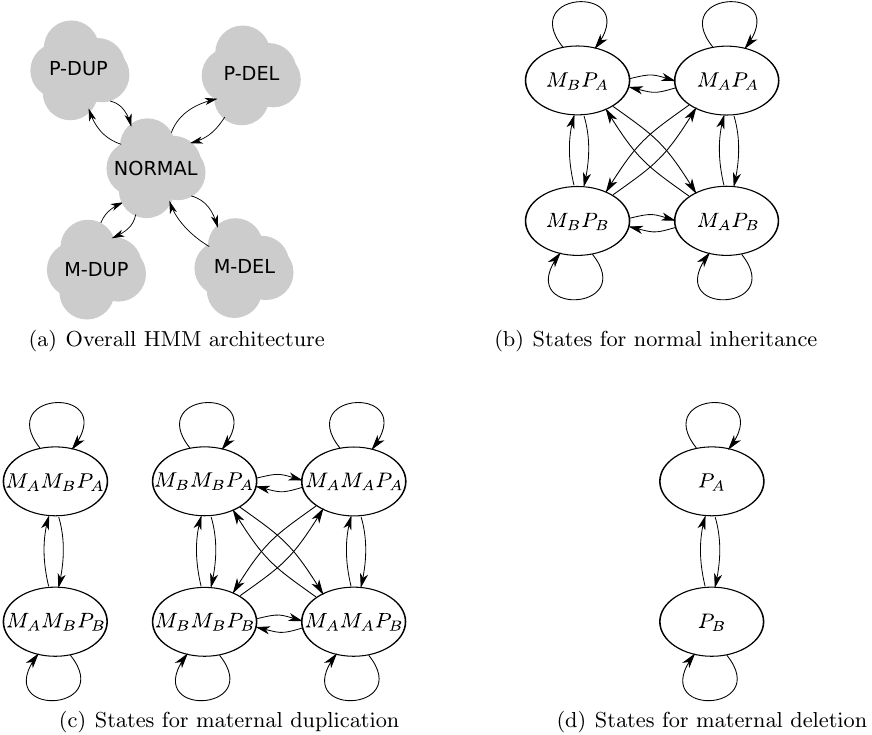
\includegraphics[width = 0.95\textwidth]{hmm}
\caption{Hidden Markov model used for CNV inference. We do not allow two CNVs to be adjacent, thus the switching always has to go through normal inheritance state ``1M 1P''.}\label{fig:hmm}
\end{figure}

%The HMM as depicted in Figure \ref{fig:hmm} is in a more general form, when we allow for different transition probabilities, depending on the given SNP site. This is useful if we want to model for non-uniform distance between individual SNPs. However in this project we assume uniform distribution and thus the transition probabilities are independent of actual position.

\todo[inline]{where to put description of data we use, phasing, etc? ..a new section "Materials"?}